%%%%%%%%%%%%%%%%% Classe che determina il tipo di documento %%%%%%%%%%%%%%%%%%%%%%
%\documentclass[a4paper,12pt,twoside,titlepage]{article}
\documentclass[a4paper,12pt,openright,twoside,titlepage]{report}
% draft <-> final Per stampare quadratini dove c'è overfull
% oneside <-> twoside Per foglio singolo, fronte/retro
% open{any<->right} Apre nuova sezione su any o a destra
% {no}titlepage Se vuoi pagina bianca dopo il titolo o meno
% twocolumn Per avere il documento su due colonne
% 10,11,12pt Dimensione del font
%%%%%%%%%%%%%%%%%%%%%%%%%%%%%%%%%%%%%%%%%%%%%%%%%%%%%%%%%%%%%%%%%%%%%%%%%%%%%%%%%

%%%%%%%%%%%%%%%%%%%%%%%%%%%%%%%%%%%%%%%%%%%%%%%%%%%%%%%%%%%%%%%%%%%%%%%%%%%%%%%%%
% File Che contiene nuovi comandi definiti da me e altre impostazioni
% Per aggiungere un nuovo comando/pacchetto/roba "globale" aggiungerla
% in questo file.
\usepackage{config/impostazioni-tesi}
%%%%%%%%%%%%%%%%%%%%%%%%%%%%%%%%%%%%%%%%%%%%%%%%%%%%%%%%%%%%%%%%%%%%%%%%%%%%%%%%%

%%%%%%%%%%%%%%%%%% Qualche comandino ganzo pronto per l'uso %%%%%%%%%%%%%%%%%%%%%
%	* \input{RelativePath/NoSpaces/File.tex} -> Include il file
%	* Comandi per le citazioni:
%	**	\textcite	-> quando la citazioneè parte integrante del discorso;
%	**	\parencite	-> racchiude la citazione fra parentesi;
%	**	\footcite	-> mette la citazione in una nota;
%	**	\supercite	-> (solo per schemi numerici) mette la citazione in apice;
%	**	\fullcite	-> mette come citazione l’intera voce bibliografica.
%%%%%%%%%%%%%%%%%%%%%%%%%%%%%%%%%%%%%%%%%%%%%%%%%%%%%%%%%%%%%%%%%%%%%%%%%%%%%%%%%

%%%%%%%%%%%%%%% Convenzioni che voglio adottare nel documento %%%%%%%%%%%%%%%%%%%
% Il comando \label va usato come segue:
%	* Ogni elemento di suddivisione logica avrà la sua label di riconoscimento
%	  e le label saranno fatte così:
%		\label{sec:RiferimentoSectionEsterna} per le sezioni di livello maggiore
%		\label{sec:RiferimentoSezioneEsterna:Sottosezione}
%		\lbale{sec:RiferimentoSezioneEsterna:Sottosezione:Sotto-Sottosezione}
%	* Ogni tabella avrà la sua label di riconoscimento e le label saranno
%	  fatte così:
%		\label{tbl:RiferimentoDellaTabella}
%	* Ogni immagine avrà la sua label che sarà così:
%		\label{fig:RiferimentoDellaFigura}
%	* Ogni equazione avrà la sua label che sarà così:
%		\label{eqn:LabelDellaEquazione}
%		N.B: le equazioni si riferiscono con \eqref
%%%%%%%%%%%%%%%%%%%%%%%%%%%%%%%%%%%%%%%%%%%%%%%%%%%%%%%%%%%%%%%%%%%%%%%%%%%%%%%%%


\begin{document}
%\frontmatter %<< questa c'è con book

\begin{titlepage}
\begin{center}
\begin{LARGE}
\textbf{UNIVERSIT\`A DEGLI STUDI DI PISA}\\
\vspace{10pt}
\end{LARGE}

% \begin{large}
% \textsc{Facolt\`a di Scienze Matematiche Fisiche Naturali}\\
% \end{large}
% \vspace{10pt}

\begin{large}
\textsc{Dipartimento di Informatica} \\
\vspace{10pt} \textsc{Corso di Laurea in Informatica}
\end{large}

\vspace{1cm}

\begin{figure}[htbp]
\begin{center}

\includegraphics[angle=0, height=4cm]{Grafica/cherubino.pdf}
\end{center}
\end{figure}

%%Se trovo un cherubino vettoriale con filigrana uso piuttosto quella sotto
%\AlCentroPagina{Grafica/cherubino-grigio.eps}

\begin{Large}
\begin{center}
\textbf{Porting di metodi multigrid per problemi di grafo in C++}
\end{center}
\end{Large}

\ \\
\begin{Large}
\textsl{Relazione Finale di Tirocinio}
\end{Large}
\\

\ \\ \ \\
\ \\
\ \\
\ \\
%\end{center}
\begin{flushleft}
\begin{large}
\textit{Tutore interno}  \hspace{238pt} \textit{Laureando}
\\ \vspace{5pt} Prof. Antonio Frangioni \hspace{5.5cm} Alessandro Lensi
\end{large}
\end{flushleft}
\ \\
\ \\
\ \\
\ \\
\ \\
\ \\
\ \\
\ \\
\ \\
\ \\
\ \\
\ \\

\line(1, 0){338} \\
\begin{large}
\textsc{Sessione di Laurea 6 Dicembre 2013} \\
\textsc{Anno Accademico 2012-2013}
\end{large}
\end{center}
\end{titlepage}
\clearpage


\tableofcontents %Indice
%\listoffigures %Indice delle figure
%\listoftables %Indice delle tabelle
% Lo faccio l'abstract?
%\input{Capitoli/Sommario}
%%%^^^^^^^^^^^^^^^^^^^^^^
%%Comunque tra frontmatter e mainmatter ci vanno ste robe qui^^

%\mainmatter %<< questa c'è con book
%%Introduzione dove parlo di MinCostFlow e InteriorPoint
\capitolo{Introduzione}
\label{intro}

\sezione{Flusso di costo minimo e metodi Interior Point}

I problemi di flusso di costo minimo (\emph{Min Cost Flow}) costituiscono un'importante classe di problemi di ottimizzazione per i quali è utile sviluppare approcci risolutivi molto efficienti.
Le sue applicazioni sono infatti molteplici.\\
Consideriamo ad esempio un'impresa di produzione e distribuzione di un certo bene composta da diversi centri:

\begin{itemize}
	\item centri di \emph{produzione} in cui la merce, non solo transita, ma viene anche realizzata in quantità prefissata
	\item centri di \emph{distribuzione} in cui il prodotto non si limita a transitare, ma viene anche consegnato in quantità prestabilita
	\item centri di \emph{stoccaggio}  in cui il bene si limita a transitare
\end{itemize}
Com'è ragionevole pensare, gli impianti sono connessi fra loro attraverso una serie di collegamenti, ai quali è facile associare un costo di trasporto e, in determinati contesti, ulteriori informazioni circa la quantità massima e minima di prodotto trasportabile lungo essi. 

Il problema che si va ad affrontare nasce dall'esigenza di determinare il modo più economico, rispetto ad una data funzione di costo, per trasportare le merci dagli impianti di produzione verso tutti i punti di distribuzione utilizzando una data rete di trasporto.

Per slegarci dai dettagli non significativi delle applicazioni in cui sorgono questi problemi viene impiegata l’entità di rete, facilmente modellabile utilizzando i grafi.
Sia dato dunque un grafo $G=(\N, \E)$ connesso, dove $\N$ è un insieme di $n$ nodi ed $\E$ un insieme di $m$ archi. Ad ogni nodo $i \in \N$ è associato un valore reale $b_i$, che rappresenta il bilancio del singolo nodo e che può assumere valore

\begin{itemize}
\item positivo, e in tal caso $i$ è un nodo di produzione;
\item negativo, e in tal caso il nodo è un nodo distribuzione;
\item nullo, ed in questo ultimo caso il nodo è un nodo di stoccaggio.
\end{itemize}

Ad ogni arco $\varepsilon_k = (i,j)$ viene associato un peso $\w_{ij}$, determinato da una opportuna funzione $\w\colon \E\to\Rp$, che indica il costo unitario da pagare per consentire a ciascuna singola unità di merce di attraversare l'arco.
Ogni arco possiede inoltre delle capacità inferiori, $l_{ij}$, e superiori, $u_{ij}$.
Queste capacità rappresentano la quantità minima o massima di merce che deve o può attraversare ciascuno degli arco del grafo.

Nei problemi di flusso la domanda globale è uguale all'offerta globale. 
In altri termini i bilanci di tutti i nodi devono soddisfare la relazione
\begin{equation*}
\label{eqn:Bilancio}
\sum_{i \in \N} b_i = 0
\end{equation*}

Un vettore $x \in \R^n$ è un flusso sul grafo $G$ se rispetta i seguenti \emph{vincoli di conservazione del flusso}:
\begin{equation*}
\label{eqn:VincoliConservazioneFlusso}
\sum_{(j,i) \in BS(i)} x_{ji} - \sum_{(i,j) \in FS(i)} x_{ij} = b_i  \quad \forall i \in \N
\end{equation*}\\
\\
Un flusso diviene ammissibile se sono inoltre verificati i seguenti vincoli di capacità:
\begin{equation*}
l_{ij} \le x_{ij} \le u_{ij} \quad \forall (i,j) \in \E
\end{equation*}\\
\\
Dato un flusso ammissibile il suo costo è dato dalla somma dei flussi degli archi per il loro costo unitario di attraversamento:

\begin{equation*}
\sum_{(i,j)\in \E} w_{ij} x_{ij}\\
\end{equation*}\\
\\
Si arriva così alla formulazione del problema del flusso di costo minimo:
\begin{equation}
\label{eq:MCFex}
\begin{split}
\min \; \sum_{(i,j)\in \;\E}w_{ij}x_{ij} \; \\
\sum_{(j,i)\;\in BS(i)}x_{ji}\;-\sum_{(i,j)\;\in FS(i)}x_{ij}\;=\;b_i\;\;\;\;\;\;i\in \N \\
l_{ij}\leq x_{ij}\leq u_{ij} \; \; \; \; (i,j)\in \E \\
\end{split}
\end{equation}
\\
nel quale l'obiettivo è quello di minimizzare il costo totale sostenuto nel trasportare il flusso di merci dai punti in cui viene prodotto verso quelli in cui viene distribuito.\\
\\

Il problema può essere espresso in forma vettoriale come
\begin{equation}
\label{eqn:MCF-vect}
\min\{ wx : Ex = b,\, l \leq x \leq u \}
\end{equation}
dove $E$ indica la matrice di incidenza del grafo $G$, $w$ il vettore dei pesi degli archi, $u$ e $l$ i vettori delle capacità superiori ed inferiori, $b$ il vettore dei bilanci dei nodi ed $x$ il vettore dei flussi.\\
\\
Il problema del flusso di costo minimo racchiude al suo interno un vasto numero di casistiche.\\
In prima analisi, pur avendo qui discusso il caso di una rete di collegamento tra i centri di un'azienda, un problema di questo tipo può insorgere in altri tipi di rete, come una rete di comunicazione o una rete idraulica.
Non solo, una modellazione di questo tipo è applicabile anche a situazioni che a prima vista potrebbero non apparire immediatamente riconducibili a problemi di flusso.\\

Si consideri ad esempio il caso di una compagnia aerea che deve stabilire i turni del personale di terra in base al flusso di passeggeri durante le ore della giornata, rispettando le normative contrattuali che prevedono vincoli sulla durata delle turnazioni, sul numero di unità di personale ogni quantitativo prestabilito di passeggeri e sulla retribuzione dei turni.
Seppur evidentemente lontano dalla nozione di rete, è possibile ricondurre questo problema ad uno di flusso di costo minimo~\cite{Turni}.\\
\\
Istanze di questo problema emergono infine, molto spesso, anche come sottomodelli di problemi più complessi~\cite{MCF_appl}.


La grande applicabilità di questi problemi è sottolineata anche dall'enorme quantità di ricerca che è stata dedicata allo sviluppo di algoritmi efficienti per la loro risoluzione, sia attraverso la specializzazione di algoritmi di \emph{Programmazione Lineare}, come il metodo del Simplesso, che attraverso lo sviluppo di approcci ad-hoc.\\
\\
Rientrano in questa seconda categoria i metodi \emph{interior point} (IP) i quali hanno ottenuto una reputazione di algoritmi efficienti per la risoluzione di grandi istanze di problemi.\\
\\
Ad ogni iterazione di questi metodi si devono risolvere sistemi lineari della forma

\begin{equation}
\label{eqn:IP}
(E \Theta E^T ) x = b
\end{equation}
dove $E$ è fissata mentre $b \in \R^n$ e la matrice diagonale $\Theta$, di dimensioni $m \times m$ e definita positiva, dipendono dall'iterazione e dal metodo IP scelto.\\
\\
I solver \emph{general purpose} di questa famiglia utilizzano dei metodi diretti per il calcolo \emph{esatto} (a meno dell'errore di rappresentazione) della soluzione. Tipicamente viene utilizzata la fattorizzazione di Cholesky preceduta da applicazioni di euristiche di riordinamento delle colonne della matrice $E$ in modo da minimizzare il fill-in ma, in caso di reti molto grandi e sparse questo approccio risulta inefficiente poiché il fenomeno non può essere mitigato~\cite{MGM_frangio}.\\
È quindi necessario utilizzare metodi iterativi per il calcolo \emph{approssimato} della soluzione, ma questi risultano competitivi soltanto nei casi in cui la velocità di convergenza sia sufficientemente alta.\\
Rientrano tra questi metodi quelli cosidetti del \emph{gradiente coniugato precondizionato} (PCG) nei quali si risolve il sottosistema

\begin{equation}
(E_S \Theta_S E_S^T )x_S = b_S
\end{equation}
dove $E_S$ e $\Theta_S$ sono restrizioni di $E$ e $\Theta$ ottenute utilizzando un opportuno sottografo $S$ del grafo di partenza, come ad esempio un albero di copertura~\cite{KKT_frangio} o un albero brother-connected (BCT)~\cite{Prim_frangio}.\\
I metodi PCG che utilizzano questi approcci funzionano bene per la maggior parte dei casi, ma in alcune applicazioni la velocità di convergenza tende ad essere bassa.
In questi casi i metodi multigrid si presentano come una valida alternativa.\\

\clearpage
\sezione{Il metodo multigrid}

Se si analizza la velocità di convergenza dei metodi iterativi classici, come ad esempio il metodo di Jacobi o quello di Gauss-Seidel, si può notare come l'errore $e = x - \tilde{x}$, che si commette ad approssimare la soluzione $x$ con $\tilde{x}$, descresca molto rapidamente nelle prime iterazioni per poi rallentare.
Questo è dovuto al fatto che l'errore si annulla molto rapidamente nello spazio delle alte frequenze mentre persiste in quello delle basse frequenze.\\
Proprio per questa caratteristica i metodi iterativi classici tendono a far assumere all'errore una forma \emph{smooth} (figura~\vref{fig:smooth}).

\fig{Grafica/smoother.pdf}{Errore iniziale (tratteggiata) e dopo 15 passi del metodo di Gauss-Seidel (piena)}{fig:smooth}

Questa proprietà viene sfruttata dai metodi multigrid per la minimizzazione dell'errore nelle alte frequenze mentre per minimizzare quello nelle basse frequenze si usa un metodo di proiezione che prende il nome di \emph{coarse grid correction} (CGC).

Sia
\begin{equation}
\label{eqn:sisteman}
A_nx_n = b_n
\end{equation}
il sistema~\eqref{eqn:IP} riscritto in modo da evidenziare la dimensione $n$ dello spazio a cui appartiene, con $A_n = (E_n \Theta_n E_n^T )$.
E sia $\bar{x}_n$ la soluzione approssimata ottenuta utilizzando un metodo iterativo classico come smoother.
L'errore introdotto da questa soluzione è pari a
\begin{equation}
\label{eqn:erroren}
e_n = x_n - \bar{x}_n
\end{equation}
ed il residuo misura 
\begin{equation}
\label{eqn:residuon}
r_n = b_n -A_n \bar{x}_n = A_n x_n - A_n \bar{x}_n
\end{equation}
Dalle equazioni~\eqref{eqn:erroren} e~\eqref{eqn:residuon} si ottiene il nuovo sistema
\begin{equation}
\label{eqn:sistemaErrore}
A_n e_n = r_n
\end{equation}
che una volta risolto ci conduce alla soluzione esatta di~\eqref{eqn:sisteman} mediante
\begin{equation}
\label{eqn:diretta}
x_n = \bar{x}_n + e_n
\end{equation}

Il sistema~\eqref{eqn:sistemaErrore} non è più facile da risolvere rispetto all'originale~\eqref{eqn:sisteman}, ma è possibile sfruttarne un'importante caratteristica.
Applicando infatti $\nu$ passaggi di un metodo iterativo classico al sistema nella forma~\eqref{eqn:IP}, partendo da un'arbitraria approssimazione iniziale $x_0$, è possibile rendere l'errore smooth.
Tale proprietà permette di poter proiettare l'errore in modo soddisfacente su uno spazio di dimensione $k$ minore rispetto all'originale e risolvere in tale spazio il sistema~\eqref{eqn:sistemaErrore}.
Riproiettando poi nello spazio di partenza la soluzione dell'errore ottenuta nello spazio più piccolo, tramite l'equazione~\eqref{eqn:diretta}, è possibile determinare una nuova soluzione approssimata più precisa rispetto ad $\bar{x}_n$.
Il metodo multigrid (MGM) è dunque un metodo iterativo che può essere visto come la composizione di almeno due distinti metodi iterativi con comportamenti spettrali di tipo complementare.\\
\\
La procedura sopra descritta lascia ancora aperte alcune importanti questioni:
\begin{itemize}
\item come poter trasferire il residuo da uno spazio $\Omega_n$ ad uno di dimensioni inferiori $\Omega_k$;
\item come poter determinare, con lo scopo di ottenere un sistema analogo a~\eqref{eqn:sistemaErrore} ma definito su $\Omega_k$, la matrice dei coefficienti $A_k$;
\item come poter riproiettare l'errore stimato in $\Omega_k$ al livello superiore $\Omega_n$.
\end{itemize}


\sottosezione{Operatori di restringimento}
Per l'implementazione della coarse grid correction, come si è detto, è necessario determinare una funzione lineare che permetta di proiettare il residuo $r_n$ da uno spazio $\Omega_n$ ad uno di dimensioni inferiori $\Omega_k$.
Sia $G(\Omega)$ l'insieme delle funzioni definite su un generico spazio $\Omega$. L'operatore di restrizione è definito come
\begin{equation*}
R_n : G(\Omega_n) \to G(\Omega_k)
\end{equation*}
ed il residuo proiettato dallo spazio più grande a quello più piccolo è dato da
\begin{equation*}
r_k = R_nr_n
\end{equation*}
La scelta di questo operatore dipende dall'applicazione che se ne vuole fare. 
Nell'ambito della risoluzione di problemi legati alle equazioni differenziali viene adoperato il cosidetto \emph{full weight operator} per le sue ottime performance.
Nell'ambito della risoluzione di problemi di grafo invece, tale operatore non si comporta altrettanto bene~\cite{fiderio}.
Nel nostro caso è necessario scegliere operatori che mantengano la struttura di grafo della matrice dei coefficienti~\cite{MGM_frangio}.

\sottosezione{Operatori di prolungamento}
La seconda classe di funzioni di trasferimento riguarda la proiezione del vettore errore dallo spazio più piccolo $\Omega_k$ a quello di dimensioni superiori $\Omega_n$.
Definendo l'operatore di prolungamento come
\begin{equation*}
P_n : G(\Omega_k) \to G(\Omega_n)
\end{equation*}
l'errore proiettato sarà
\begin{equation*}
e_n = P_n e_k
\end{equation*}

Questa procedura, molto comune in analisi numerica, prende il nome di \emph{interpolazione}.
Come operatore di prolungamento si può utilizzare qualsiasi tecnica di interpolazione ma in genere, per la sua semplicità e per il fatto che offra risultati più che soddisfacenti, viene di solito impiegata l'interpolazione lineare~\cite{MGM_web_tut}.

L'operatore di interpolazione lineare è così definito:
\begin{equation}
e_{n,j} = 
\begin{cases}
\frac{1}{2}(e_{k,i-1} + e_{k,i}) & \text{per } j = 2i +1\\
e_{k,i} & \text{per } j=2i
\end{cases},
i = 0,\dots,k-1
\end{equation}

È utile far notare che se l'errore in $\Omega_n$ è un vettore smooth e se si conosce un'approssimazione esatta dell'errore du $\Omega_k$, allora l'interpolazione di tale approssimazione sullo spazio $\Omega_n$ è anch'essa smooth. Al contrario, se l'errore di partenza è oscillatorio, una sua buona approssimazione nel sottospazio ne produrrà, dopo l'interpolazione, una non molto accurata.
Poiché l'interpolazione è necessaria nella CGC si può concludere che tale processo è tanto più efficace quanto l'errore di partenza è smooth.
Questo ci consente di apprezzare la complementarietà delle due fasi del multigrid.
Il rilassamento su $\Omega_n$, ottenuto con un metodo iterativo classico, elimina velocemente i componenti oscillatori dell'errore lasciando un errore smooth. L'interpolazione lineare, per via della bontà dell'errore, assumendo che il sistema~\eqref{eqn:sistemaErrore} venga risolto in maniera accurata sul sottospazio $\Omega_k$, trasferisce correttamente l'errore all'indietro sul sottospazio $\Omega_n$.\\
Proprio per il fatto di essere complementari i due metodi, che presi singolarmente richiederebbero un numero elevato di iterazioni per raggiungere la convergenza, combinati insieme risultano particolarmente veloci.


\sottosezione{Matrice dei coefficienti}

Quel che rimane da determinare per risolvere l'equazione del residuo~\eqref{eqn:sistemaErrore} nel sottospazio $\Omega_k$ è la matrice dei coefficienti ristretta $A_k$. Tale scelta deriva dalla condizione di Galerkin~\cite{MGM_tutorial}:
\begin{equation}
A_k = R_n A_n P_n
\end{equation}

Adesso che abbiamo definito, in linea di principio, tutti gli strumenti necessari possiamo descrivere formalmente il funzionamento del CGC.\\
\\
Sia $\bar{x}_n$ una qualsiasi approssimazione delle soluzione del sistema~\eqref{eqn:sisteman}. Tale approssimazione può essere corretta mediante la seguente procedura:


\begin{algorithm}
\caption{$\bar{x}_n = \text{CGC}(\bar{x}_n,b_n)$}
\label{alg:CGC}
\begin{algorithmic}[1]
\State Calcola il residuo $r_n = b_n - A_n\bar{x}_n$ sullo spazio $\Omega_n$
\State Restringi il residuo nel sottospazio $\Omega_k$ con $r_k = R_nr_n$
\State Ricava $A_k = R_n A_n P_n$
\State Risolvi $e_k = A_k^{-1}r_k$ su $\Omega_k$
\State Interpola l'errore su $\Omega_n$ con $e_n = P_ne_k$
\State Correggi l'approssimazione iniziale $\bar{x}_n = \bar{x}_n + e_n$
\end{algorithmic}
\end{algorithm}

\sottosezione{Metodo Two-Grid}

Combinando un metodo iterativo classico alla procedura di coarse grid correction è possibile definire il metodo \emph{two grid} (TGM): si applicano prima alcuni passi di un metodo iterativo per ammorbidire l'errore, poi la coarse grid correction ed infine di nuovo alcuni passi di un metodo iterativo, eventualmente anche diverso dal precedente per ammorbidire ulteriore l'errore commesso dalla CGC. Il primo metodo iterativo prende il nome di \emph{pre-smoother} ed il secondo quello di \emph{post-smoother}.
Data quindi una soluzione iniziale $\bar{x}_0$ se ne può ottenere una migliore $\bar{x}_n$ tramite la seguente procedura:
\begin{algorithm}
\caption{$\bar{x}_n = \text{TGM}(\bar{x}_0)$}
\label{alg:TGM}
\begin{algorithmic}[1]
\State Rilassa $\nu_{\text{pre}}$ volte il sistema $A_n \bar{x}_o = b_n$ su $\Omega_n$ ottenendo una approssimazione $\bar{x}_n$
\State $\bar{x}_n = CGC(\bar{x}_n,b_n)$
\State Rilassa $\nu_{\text{post}}$ volte il sistema $A_nx_n = b_n$ su $\Omega_n$ partendo dalla soluzione $\bar{x}_n$
\end{algorithmic}
\end{algorithm}

\sottosezione{$\mu$-Cycle Scheme}

L'algoritmo~\vref{alg:CGC} lascia aperta un'incombente questione procedurale: come risolvere il sistema del sottospazio
\begin{equation}
A_ke_k = r_k
\end{equation}

La risposta non può che trovarsi nella ricorsione. È facile intuire infatti come sia possibile applicare il TGM anche all'equazione del residuo definita su $\Omega_k$ e portarsi su un nuovo sottospazio $\Omega_p$ di dimensioni inferiori.
Tale procedura può essere applicata fino ad ottenere un sottospazio $\Omega_l$ di dimensioni sufficientemente piccole, in cui il sistema possa essere risolto in maniera diretta. La soluzione così ottenuta, una volta interpolata, viene utilizzata per correggere l'approssimazione precedente. Questo procedimento viene ripetuto per ogni spazio intermedio fino a ritornare nello spazio di partenza $\Omega_n$.

La procedura si può riassumere come segue:
\begin{algorithm}
\caption{$\bar{x}_n = MGM\mu(\bar{x}_i, b_i)$}
\label{alg:MGM}
\begin{algorithmic}[1]
\If{ $(i == L)$ }\Comment{l è l'ultimo livello}
	\State $b_i = A_i^{-1}x_i$
\Else
	\State Rilassa $\nu_{pre}$ volte $A_ix_i =b_i$ partendo da $\bar{x}_i$
	\State Calcola il residuo $r_i = b_i - A_i \bar{x}_i$
	\State Applica $r_{i+1} = R_i r_i$
	\State Chiama $\bar{x}_i = MGM_{\mu}(\bar{x}_{i+1},b_{i+1})$ $\mu$ volte
	\State Correggi $\bar{x}_i = \bar{x}_i + e_i$
	\State Rilassa $\nu_{post}$ volte $A_ix_i = b_i$ partendo da $\bar{x}_i$
\EndIf
\end{algorithmic}
\end{algorithm}

Il parametro $\mu$ di questo metodo serve per definire diversi schemi di chiamate ricorsive. Nella pratica si utilizzando solo $\mu = 1$, che produce un V-cycle, e $\mu = 2$ che produce un W-cycle (figura~\vref{fig:cycle}).


\fig{Grafica/Cycles.pdf}{Rappresentazione grafica di un V-cycle e di un W-Cycle}{fig:cycle}




\capitolo{LAMG: Lean Algebraic MultiGrid}
\label{cap:LAMG}

Quella del \emph{multigrid algebrico} (AMG) è una classe di risolutori di sistemi lineari che trae le sue origini negli anni '80 ed ancora sotto attivo sviluppo.
Questi metodi si dividono in due fasi principali.\\
Nella prima, detta di \emph{setup}, viene costruita una gerarchia di matrici sempre più coarse, cioè di dimensioni minori, senza utilizzare informazioni geometriche deducibili dall'istanza di problema, come invece avviene nei metodi del \emph{multigrid geometrico}.\\
Nella seconda fase, detta di \emph{solve}, si effettuano dei cicli multigrid come quelli descritti nell'algoritmo~\vref{alg:MGM}.

LAMG è un algoritmo di tipo AMG che risolve sistemi di equazioni lineari della forma
\begin{equation*}
Ax = b
\end{equation*}
dove la matrice dei coefficienti $A$ è una matrice laplaciana di grafo.
Può trovare quindi applicazione come metodo iterativo nella risoluzione dei sistemi nella forma~\eqref{eqn:IP} legati ai problemi di MCF e, più in generale per la risoluzione di problemi di grafo.\\
Sia dato un grafo $G=(\N,\E,\w)$, dove $\N$ è un insieme di nodi, $\E$ un insieme di archi e $\w$ la funzione che assegna un peso positivo a ciascuno degli archi di $\E$. \\
Definiamo la matrice diagonale $D$ avente come elementi diagonali la somma dei pesi degli archi di ciascun nodo
\begin{equation}
d_i = \sum_{j \in \N,\,j \ne i} \w_{i,j} \quad \forall i \in \N
\end{equation}
Definiamo inoltre la matrice di adiacenza pesata del grafo $G$ come
\begin{equation}
a_{i,j} = 
\begin{cases}
\w_{i,j} & \text{se } (i,j) \in \E\\
0 							& \text{altrimenti}
\end{cases}
\end{equation}
La matrice Laplaciana di grafo è data da
\begin{equation}
L = D - A
\end{equation}
Tale matrice è simmetrica e a predominanza diagonale.
\sezione{Le scelte di LAMG}
Nel capitolo~\vref{intro} si è visto come ciascuna implementazione multigrid debba effettuare principalmente due scelte:
\begin{itemize}
\item Scegliere il metodo iterativo da utilizzare come smoother
\item Scegliere che tipo di operatore di restringimento utilizzare per poter proiettare il residuo dallo spazio $\Omega_n$ al sottospazio $\Omega_k$
\end{itemize}

La scelta del primo ricade sul metodo di Gauss-Seidel poiché richiede meno memoria rispetto, ad esempio, al metodo di Jacobi.

Si consideri la decomposizione della matrice $A$ data da
\begin{equation*}
A = D - B - C
\end{equation*}
dove
\begin{equation*}
d_{i,j} =  
\begin{cases}
a_{i,j} & \text{se } i = j\\
0 & \text{se } i \ne j
\end{cases},\,
b_{i,j} =
\begin{cases}
-a_{i,j} & \text{se } i > j\\
0 & \text{se }i \leq j
\end{cases},\,
c_{i,j} =
\begin{cases}
0 & \text{se } i \geq j\\
-a_{i,j} & \text{se } i < j
\end{cases}\end{equation*}

Scegliendo $M = D - B$ e $N = C$ si può riscrivere il sistema di partenza come 
\begin{equation*}
(M- N)x = b
\end{equation*}
ovvero
\begin{equation*}
Mx = Nx + b
\end{equation*}
da cui segue
\begin{equation*}
x = M^{-1}Nx+M^{-1}b
\end{equation*}  

Questo sistema, posto
\begin{equation*}
G = M^{-1}N = (D-B)^{-1}C
\end{equation*}
e scelta una soluzione iniziale $x^{(0)}$, da luogo alla successione
\begin{equation}
\label{eqn:GS}
x^{(k)} = Gx^{(k-1)}+(D-B)^{-1}b
\end{equation}
Per descrivere come viene implementato il metodo di Gauss-Seidel conviene prima trasformare la~\eqref{eqn:GS} così
\begin{equation*}
\begin{split}
(D-B)x^{(k)} &= Cx^{(k-1)} + b\\
Dx^{(k)} &= Bx^{(k)} + Cx^{(k-1)} + b\\
x^{(k)} &= D^{-1}Bx^{(k)}+D^{-1}x^{(k-1)} + D^{-1}b
\end{split}
\end{equation*}

Il metodo di Gauss-Seidel viene allora implementato nel modo seguente
\begin{equation}
x_i^{(k)} = \frac{1}{a_{ii}} \bigg[b_i - \sum_{j=1}^{i-1} a_{ij}x_j^{(k)} - \sum_{j=i+1}^{n} a_{ij}x_j^{(k-1)} \bigg],\, i=1,2,\dots,n
\end{equation}

Il vantaggio fondamentale di questo metodo è che per calcolare le componenti del vettore $x^{(k)}$ si utilizzano anche le componenti già calcolate dello stesso vettore. Quindi è sufficiente disporre di un solo vettore in cui si sostituiscono le componenti via via che vengono calcolate.
Inoltre la convergenza è garantita se applicato alla matrice laplaciana poiché la predominanza diagonale di quest'ultima fornisce una condizione \emph{sufficiente}~\cite[110]{Toporagno}.\\
\\
Per quanto riguarda la seconda scelta LAMG utilizza una combinazione di due metodi per costruire, ad ogni livello, l'operatore di restrizione.

Il primo, detto \emph{Aggregation}, crea la matrice più coarse, cioè diminuisce la dimensione della matrice $A$, aggregando i nodi del livello $\Omega_n$ secondo un criterio di prossimità che prende il nome di \emph{affinity}.\\
\\
Il secondo, detto \emph{Low Degree Elimination}, ha lo scopo di eliminare dal grafo quella parte che non può essere aggregata in maniera efficace dall'altro metodo.
Nella sezione~\vref{subsec:AggeLDE} vedremo nel dettaglio il funzionamento di questi due metodi.

Il sistema del livello più basso $L$ viene risolto utilizzando il metodo di Gauss-Seidel, se la convergenza risulta essere veloce, oppure utilizzando un metodo diretto su un sistema aumentato~\cite{lamg_Report}.

\sezione{Operatori di restringimento di LAMG}
\label{subsec:AggeLDE}

Conforme agli altri metodi multigrid, LAMG costruisce come prima cosa una gerarchia di $L$ sistemi $A_l x_l = b_l$, detti livelli, di dimensioni sempre inferiori rispetto al precedente. Il sistema $A_lx_l = b_l$ corrisponde a quello di partenza. 
Gli altri livelli $i\geq 2$ sono ottenuti con il metodo di Galerkin utilizzando come matrice $R$ o una matrice di eliminazione, e allora il livello corrispondente sarà di \emph{Elimination}, o di aggregazione, e allora il livello sarà di \emph{Aggregation}.
Tali tecniche vengono alternate per la generazione della gerarchia dei livelli.\\
\\
\sottosezione{Low Degree Elimination}
\begin{figure}
\centering
\begin{tabular}{cccc}
\toprule
$|\E_i|$ & $\Delta_m$ & Prima dell'eliminazione & Dopo l'eliminazione \\
\midrule
$1$ & $-1$ & 
\includegraphics[height=0.015\textheight]{Grafica/el-A} & 
\includegraphics[height=0.015\textheight]{Grafica/el-B}\\
\midrule
$2$ & $-1$ & 
\includegraphics[height=0.015\textheight]{Grafica/el-C} & 
\includegraphics[height=0.015\textheight]{Grafica/el-D}\\
\midrule
$3$ & $0$ & 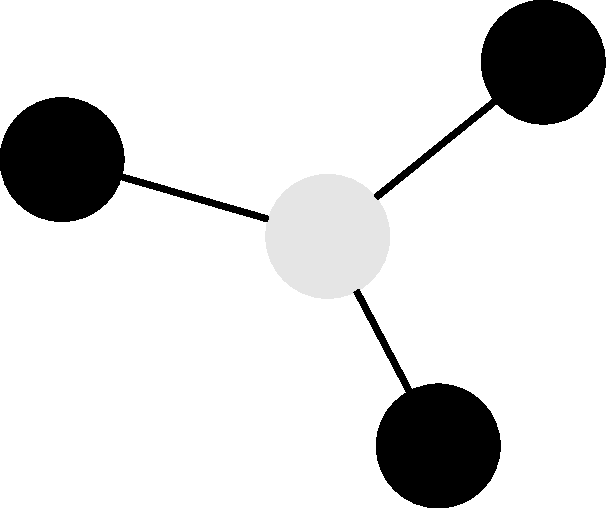
\includegraphics[height=0.04\textheight]{Grafica/el-E} & 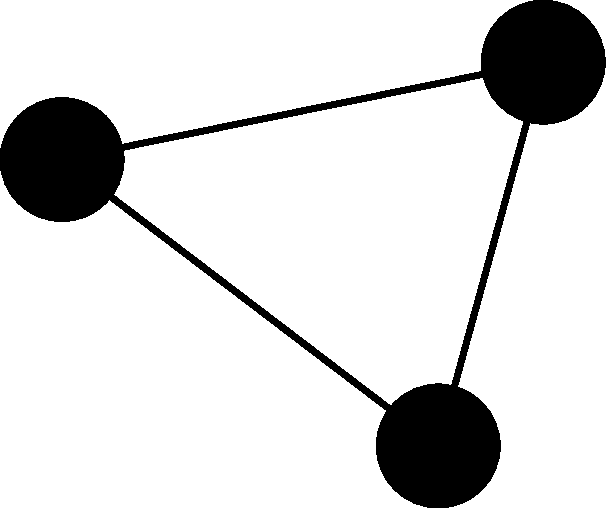
\includegraphics[height=0.04\textheight]{Grafica/el-F}\\
\midrule
$4$ & $+2$ & 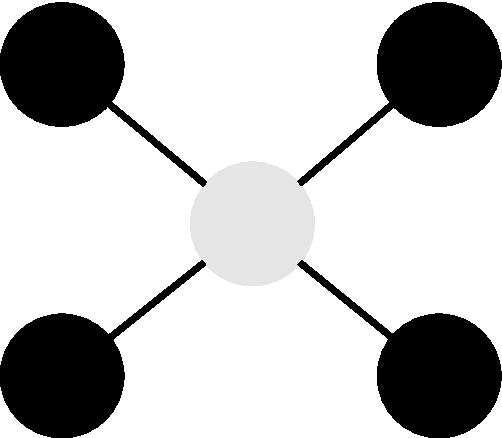
\includegraphics[height=0.04\textheight]{Grafica/el-G} & 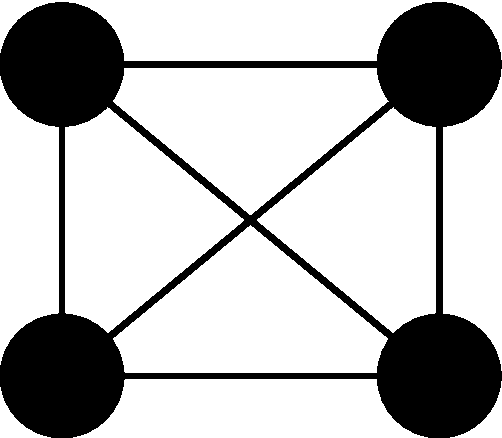
\includegraphics[height=0.04\textheight]{Grafica/el-H}\\
\midrule
\end{tabular}
\caption{Come viene modifica la porzione di grafo interessata prima e dopo l'eliminazione dei nodi candidati (nodi in grigio). $\Delta_m$ è la variazione massima del numero di archi.}
\label{tbl:elimino}
\end{figure}

La creazione di un livello Elimination avviene eliminando dall'insieme dei nodi $\N$ un sottoinsieme $\F$ di nodi indipendenti di grado $|\E_i| \leq 4$.
L'eliminazione di un singolo nodo comporta la connessione di tutti i suoi vicini. 
L'eliminazione di un nodo con grado $|\E_i| \leq 3$ non comporta l'aggiunta di nessun arco, e dunque nessun fill-in per la matrice dei coefficienti, così come riassunto in figura~\vref{tbl:elimino}.
Quando $|\E_i| = 4$, $m$ può aumentare di al più $2$ e questo, nella pratica, è accettabile perché l'alternativa, impraticabile perché costosa, sarebbe quella di monitorare tutti i futuri cambiamenti di $m$ e decidere se eliminare il nodo solo nel caso che questo non comporti maggiori aumenti.
Valori più grandi di $\E_i$ risultano in un impratico fill-in della matrice dei coefficienti.
\\
La selezione dei nodi in $\F$ avviene con una visita su tutti i nodi con grado $|\E_i| \leq 4$. Quando un nodo viene marcato come \textsc{fnode} tutti i suoi vicini vengono marcati come non eleggibili (\textsc{noteliminated}) in modo da garantire l'indipendenza di tale insieme (algoritmo~\vref{alg:LowDegreeNodes}).

Consideriamo ora l'insieme $\C = \N \setminus \F$, cioè l'insieme dei nodi high-degree che rimangono dopo aver eliminato quelli low-degree. Il sistema di partenza $\matr{Ax} = \matr{b}$ si riduce dunque al sistema complementare di Schur definito come

\begin{equation}
\label{eqn:SchurComplementSystem}
A^cx_{\C} = b^c \text{ dove }%
A^c = RAP \text{, }%
b^c = Rb \text{, }%
R  = \Pi (-A_{\F\C}^T A_{\F\F}^{-1},I_{\C})
\end{equation}
dove $\Pi$ è una matrice di permutazione tale che $\Pi^Tx$ mostra tutti i valori dei nodi di $\F$ e poi tutti i valori dei nodi in $\C$.
\eqref{eqn:SchurComplementSystem} è un sistema Laplaciano più piccolo, per il quale vengono eseguiti ulteriori passaggi di eliminazione utilizzando l'algoritmo~\vref{alg:Elimination} fino a quando $\abs{\F}$ non diventa sufficientemente piccolo.

\begin{algorithm}
\caption{$\F = LowDegreeNodes(\matr{A})$}\label{alg:LowDegreeNodes}
\begin{algorithmic}[1]
\State $\N\gets nodes(\matr{A})$, $n \gets size(\matr{A}), \U \gets \Set{u\in\N : 1 \le \abs{\E_u} \le 4}$
\State For each $u \in \U, visited(u) \gets \text{\textsc{notvisited}}$
\For{each $u\in\U$}
	\If{$visited(u) = \text{\textsc{notvisited}}$}
		\If{$\nexists v \in \E_u : visited(v) = \text{\textsc{fnode}}$}\Comment{$u$ può essere eliminato}
			\State $visited(u) \gets \text{\textsc{fnode}}$
			\State For each $v \in \E_u, visited(v) \gets \text{\textsc{noteliminated}}$
		\Else\Comment{$u$ ha un vicino che è in $\F$}
			\State $visited(u)\gets\text{\textsc{noteliminated}}$
		\EndIf
	\EndIf
\EndFor
\State $\text{return } \F = \Set{u \in \U : visited(u) = \text{\textsc{fnode}}}$
\end{algorithmic}
\end{algorithm}

Se nessun nodo viene eliminato in questa fase di eliminazione allora l'attuale livello rimane il coarsest, altrimenti la coppia $(A^c, R)$ definisce il prossimo livello $l+1$.

In entrambi i casi si procede con la fase di aggregazione per tentare di ridurre la dimensione del vecchio livello, o del nuovo appena creato.\\
\\
\begin{algorithm}
\caption{$[\A^c, \Pp, \Q, \Set{\Pp_i,\Q_i}_{i=1}^q] = Elimination(\A)$}\label{alg:Elimination}
\begin{algorithmic}[1]
\State $\A^c \gets \A, \N^c \gets nodes(\A), n_c \gets \abs{\N^c}, \Q \gets \matr{0}_{n_c}, \Pp \gets \matr{I}_{n_c}, q \gets 0$
\While{$n_c > 1$}
	\State $\F \gets LowDegreeNodes(\A^c)$
	\If{ $(\abs{\F} < 0.01n_c)$}
		\State return $[\A^c, \Pp, \Q, \Set{\Pp_i,\Q_i}_{i=1}^q]$
	\EndIf
	\State $q \gets q+1, \C \gets \N \setminus \F$
	\State $\Pie \gets \text{una matrice di permutazione che ordina }\N^c \text{ come } (\F,\C)$
	\State $\Q_i \gets \Pie \cdot \text{diag} \Set{(\A_{\F\F}^c)^{-1},\0_\F },\,\matr{R} \gets (\0_\F, \I_\C)$
	\State $ \Pp_i \gets \Pie \cdot ( -(\A_{\F\C}^c)^T(\A_{\F\F}^c)^{-1},\I_\C)^T$
	\State $\Q \gets \Q + \Pp\Q_i\Rr, \Pp \gets \Pp_i\Pp, \A^c \gets \Pp^T\A^c\Pp, \N^c \gets nodes(\A^c), n_c \gets \abs{\N^c}$
\EndWhile 
\end{algorithmic}
\end{algorithm}

\sottosezione{Aggregation}

Per la creazione efficace di un livello Aggregate è determinante definire quali elementi di $\N$ siano \emph{prossimi}.
I metodi multigrid tipicamente utilizzano misure di prossimità che si basano sui pesi degli archi per operare questa scelta:

\begin{equation}
\label{eqn:ClassicalAMGProximity}
\frac{1 - \abs{\w_{uv}}}{ \max \{ \max_s \abs{\w_{us}} , \max_s \abs{\w_{sv}} \}}
\end{equation}

Questa misura funziona molto bene nel caso si trattino problemi legati alle equazioni differenziali ellittiche alle derivate parziali, dove si possono utilizzare anche informazioni di natura geometrica, ma porta a decisioni di aggregazione infelici nel caso di grafi non locali.

Ad esempio in un grafo a griglia con un arco extra che connette nodi distanti $u$ e $v$ questi rischiano di diventare prossimi e possono essere aggregati (vedi figura~\vref{fig:Agg}a).
A meno che il peso di tale arco non sia molto grande, questo comportamento non è desiderabile perché produce un'aggregazione di nodi che corrispondono a maglie della griglia non correlate tra loro.
Questo è un grande problema poiché i grafi a griglia che compaiono nei problemi GMG discretizzano oggetti reali su cui vogliamo fare simulazioni di fluidodinamica, come ad esempio un alettone della Ferrari.\\
Se due punti della griglia che sono fisicamente lontani vengono aggregati dal metodo accade che divengano correlate due parti dell'alettone che in realtà non lo sono e la simulazione produce quindi dei risultati non corretti.\\
Questo problema è stato superato con l'introduzione della distanza algebrica:
\begin{equation}
\label{eqn:AlgebraicDistance}
\max_{k=1}^K \abs{ x_u^{(k)} - x_v^{(k)} }
\end{equation}

Tale misura consente di aggregare due nodi $u$ e $v$ solo se c'è una forte correlazione tra di loro nel dominio degli smooth error vectors.
Viene effettuato un test di correlazione scegliendo $K$ \emph{Test Vector} (TV) come campione di questo spazio.
Ogni test vector è il risultato dell'applicazione di $\nu$ passaggi di rilassamento al sistema omogeneo $\matr{Ax}=\matr{0}$, partendo da valori casuali in $[-1,1]$.\\
Con la distanza algebrica si risolve il problema precedentemente sollevato ma non il seguente.
Se il grafo contiene due nodi hub $u$ e $v$, cioè due nodi fortemente connessi, succede che per ogni $k$ il valore $x_u^{(k)}$ è una media di valori casuali, calcolata su un insieme di vicini molto grande, la cui dimensione aumenta con il numero di passi di rilassamento, e che dunque è piccola. Analogamente $x_v^{(k)}$ è un valore piccolo, dunque la coppia $(u,v)$ viene considerata come vicina anche se in realtà tali nodi possono essere distanti (figura~\vref{fig:Agg}b).

\begin{figure}%
\centering
\subfloat[][\emph{Una griglia 2D con un arco extra}.]{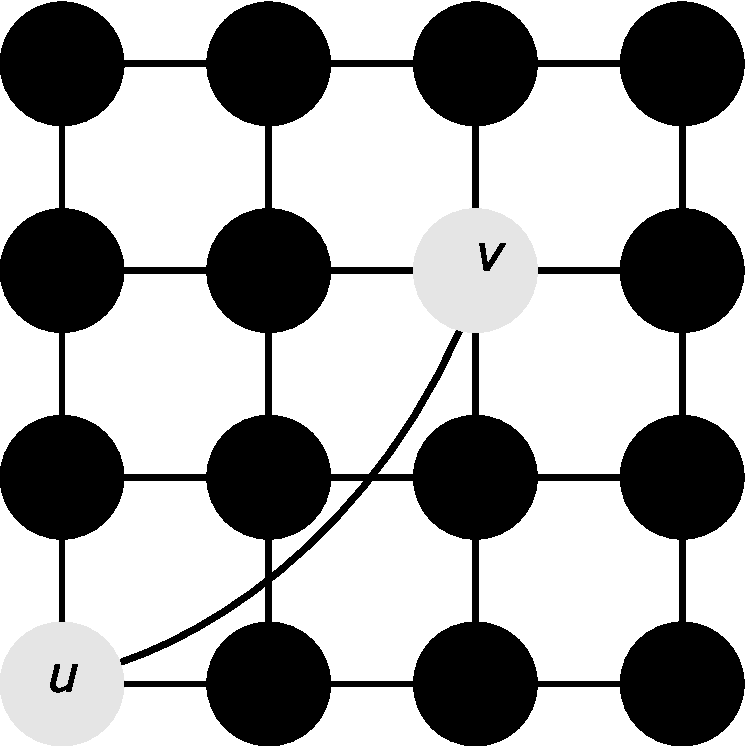
\includegraphics[width=0.25\textwidth]{Grafica/aggregazioniPericolose}} \label{fig:AggA} \quad
\subfloat[][\emph{Due hub connessi. Un hub è un nodo high-degree}.]{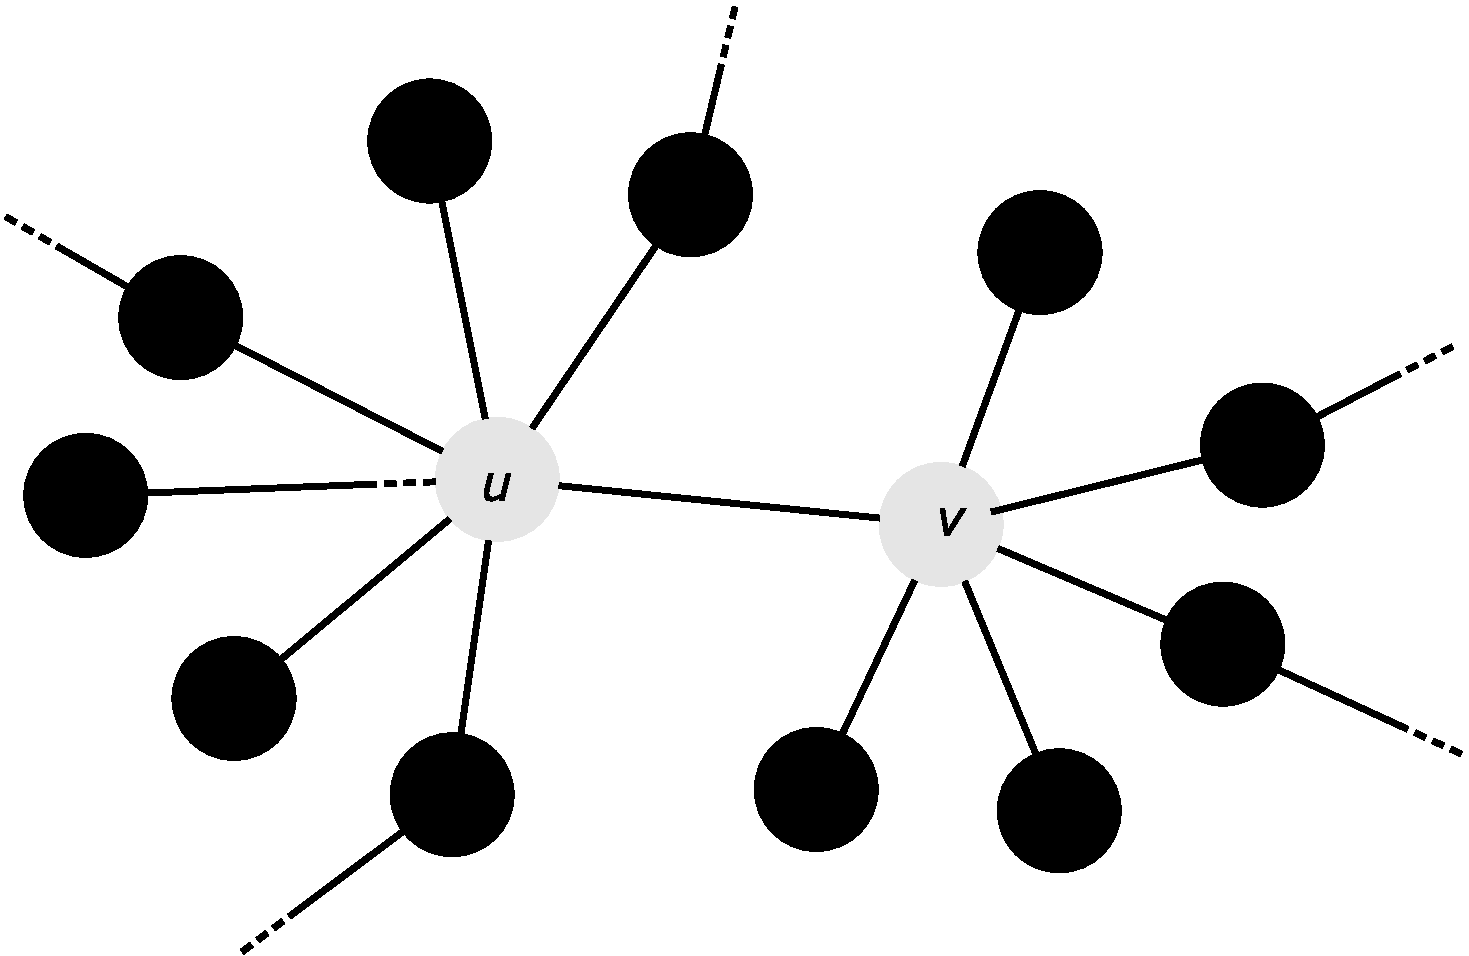
\includegraphics[width=0.35\textwidth]{Grafica/aggregazioniPericolose2}} \label{fig:AggB}\\
\caption{Esempi di aggregazioni pericolose}
\label{fig:Agg}%
\end{figure}%

La misura di prossimità introdotta in LAMG, la \emph{affinity}, gestisce in maniera corretta sia i due casi visti precedentemente sia altri tipi di topologie.
La affinity $c_{uv}$ tra i due nodi $u$ e $v$ è definita come la “bontà'' nell'approssimare  il modello lineare $x_v \approx px_v$ coi valori dei test vector:

\begin{equation}
\label{eqn:Affinity}
c_{uv} = 1 - \frac{ \abs{( X_u, X_v) }^2}{(X_u,X_u)(X_v,X_v)}
\end{equation} 
con $c_{uu} = 0$, $0\le c_{uv} \le 1$ e $c_{uv} = c_{vu}$ e dove
\begin{equation*}
(X,Y) = \sum_{k=1}^K x^{(k)}y^{(k)}
\end{equation*}
mentre 
\begin{equation*}
X_u = (x_u^{(1)}, \dots, x_u^{(K)})
\end{equation*} 

La affinity misura la distanza tra due nodi: più \emph{piccolo} è $c_{uv}$ più \emph{vicini} sono i nodi $u$ e $v$.\\
\\
La creazione di un livello Aggregate equivale a partizionare l'insieme dei nodi $\N$ in $n_c$ sottoinsiemi disgiunti $\{\T_U\}_{U\in\N^c}$, detti \emph{aggregati}.$\T_U$ è l'insieme di $e_u$ interpolato a partire da $e_U^c$ ed $\N^c = \{1,\dots,n_c\}$.
Ogni aggregato consiste in un nodo \emph{seed} e zero o più nodi \emph{associati} (figura~\vref{fig:seeds}).

\begin{figure}%
\centering
\subfloat[][\emph{Il grafo di partenza}.]{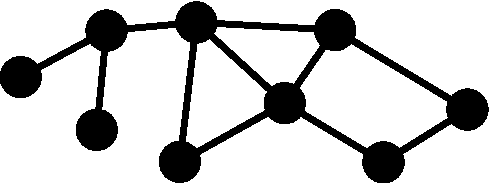
\includegraphics[width=0.25\textwidth]{Grafica/aggr-A}} \quad
\subfloat[][\emph{Una aggregazione. I nodi seed sono indicati in grigio}.]{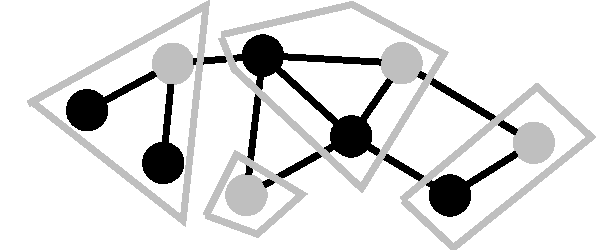
\includegraphics[width=0.25\textwidth]{Grafica/aggr-B}} \\
\subfloat[][\emph{Ciascun aggregato corrisponderà ad un nodo nel grafo coarse}.]{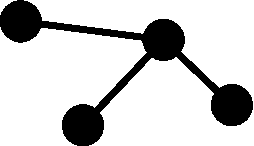
\includegraphics[width=0.20\textwidth]{Grafica/aggr-C}} \\
\caption{Risultati di una aggregazione}
\label{fig:seeds}%
\end{figure}%

Gli aggregati ideali hanno una forte affinity tra di loro, ed una affinity coi rimanenti vicini più debole. 
A tale scopo si definiscono le seguenti regole di aggregazione:

\begin{enumerate}
\item Ogni nodo può essere associato con un solo seed;
\item Un seed può essere associato solo con se stesso;
\item Aggrega prima nodi con affinity minore (più vicini) e poi quelli con affinity maggiore (più lontani);
\item Un nodo hub deve diventare un seed.
\end{enumerate}

Le regole 1-2 hanno lo scopo di evitare associazioni transitive tra seed distanti. Senza di queste si potrebbero creare degli aggregati con connessioni interne deboli tra lunghe catene di seed.
La regola 3 garantisce connessioni locali.
La regola 4, infine, ha lo scopo di evitare decisioni computazionalmente costose derivanti dall'attraversamento del grande insieme di vicini del nodo hub.\\
Un hub è definito come un nodo il cui grado è sufficientemente più alto della media pesata di quello dei suoi vicini:
\begin{equation}
\label{eqn:HubNode}
\abs{\E_u} \ge \frac{ 8\sum_{v\in\E_u} \abs{\w_{uv}}\abs{\E_v} }{ \sum_{v\in\E_u}\abs{\w_{uv}} }
\end{equation}


\begin{algorithm}
\caption{$S = aggregate(\A,\matr{X},\alpha_{\max},I_{\max})$}\label{alg:Aggregate}
\begin{algorithmic}[1]
\State $I_{\max} \gets 2,\, B(1..I_{\max}) \gets \infty,\, n \gets size(\A)$
\State $n_c \gets n,\, \alpha \gets 1,\, i \gets 0,\, \delta \gets 0.9 $
\State $\matr{C} \gets (c_{uv})_{u,v} \text{ where } c_{uv} \gets$ equazione~\eqref{eqn:Affinity} con $\matr{X}$ come test vector, $\forall (u,v) \in \E$
\State For each $u \in \U,\, status(u) \gets \textsc{undecided},\, aggregateSize(u) \gets 1$\label{alg:Aggregate:1}
\State For each $u \in \Set{u : \abs{\E_u} \ge 8\cdot median({\E_v}_v)}, status(u) \gets 0$\label{alg:Aggregate:2}
\While{$(\alpha \ge \alpha_{\max}) \text{ and } (i < I_{\max})$}\Comment{Loop principale di aggregation}
	\State $ i \gets i+1,\, \delta \gets 0.6\delta$
	\State $aggregationStage(status,\A,n_c,\matr{C},\matr{X},aggregateSize,\delta)$
	\State $\alpha \gets n_c/n,\, B_i \gets (1- \alpha \text{ if } \alpha \le \alpha_{\max} \text{ otherwise } 1+ \alpha)$\label{alg:Aggregate:3}
	\State $S_i \gets status$\Comment{Salva l'insieme degli aggregati corrente}
	\State For each $u \in \Set{v:S_i(v) = \textsc{seed}},\,S_i(v) \gets v$
\EndWhile
\State $i \gets \text{argmin}(B)$\Comment{Sceglie il miglior insieme di aggregati}
\State $\text{return } S_i$
\end{algorithmic}
\end{algorithm}


\begin{algorithm}
\caption{$aggregationStage(status,\A,n_c,\matr{C},\matr{X},aggregateSize,\delta)$}\label{alg:aggregationStage}
\begin{algorithmic}[1]
\State $\matr{N} \gets \Set{c_{uv} \ge \delta\cdot\max\Set{\max_{s\ne u} c_{us}, \max_{s\ne v} c_{sv}}} $\Comment{Insieme degli strong neighbors}
\State $\matr{U} \gets \Set{u:status(u) = \text{\textsc{undecided}}}$
\For{each $u \in \matr{U}\cap\Set{u:\E_u\cap\matr{N}} = \emptyset$}\Comment{Nodi undecided con strong neighbors}
	\If{$status(u) \ne \text{\textsc{undecided}}$}\Comment{Lo stato di $u$ può cambiare nel ciclo} 
		\State continue
	\EndIf
	\State $s \gets bestSeed(\A,\matr{X},aggregateSize,\matr{N},\matr{C},u)$
	\If{$s \ne \text{\textsc{notfound}}$}\Comment{$s$ è un seed vicino, aggrega $u$ con $s$}
		\State $status(s)\gets \text{\textsc{seed}},\, status(u) \gets s,\, n_c \gets n_c - 1$
		\State For $k = 1,\dots,K \,,\, x_{uk} \gets x_{sk}$\Comment{Aggiorna i valori del TV}
		\State $aggregateSize(u),aggregateSize(s) \gets aggregateSize(s) + 1$
	\EndIf
\EndFor
\end{algorithmic}
\end{algorithm}

\begin{algorithm}
\caption{$s \gets bestSeed(\A,\matr{X},aggregateSize,\matr{N},\matr{C},u)$}
\label{alg:bestSeed}
\begin{algorithmic}[1]
\State $S \gets \matr{N} \cap \Set{ u : status(u) \in \Set{ \textsc{Undecided}, \textsc{Seed} } }$
\If{$S = \emptyset$}
	\State return \textsc{NotFound}
\Else
	\State return $\argmax{v \in S} c_{uv}$
\EndIf
\end{algorithmic}
\end{algorithm}
L'algoritmo di aggregazio richiede l'indice del ciclo multigrid $\mu$ come parametro di input.
Ogni nodo può essere marcato come \textsc{seed}~(con valore pari a $0$), \textsc{associate}~(con valore pari all'indice del seed a cui è associato) o \textsc{undecided}~(con valore pari a $-1$).

Inizialmente tutti i nodi vengono marcati come \textsc{undecided}~(riga~\ref{alg:Aggregate:1}). 

Si procede poi~(riga~\ref{alg:Aggregate:2}) ad indentificare e marcare come seed tutti i nodi hub utilizzando la formula~\eqref{eqn:HubNode}.

Poi si scartano gli archi che hanno un peso $\abs{\w_{uv}}$ molto piccolo per accelerare la velocità di convergenza è ridurre il numero di calcoli da effettuare.

I nodi che eventualmente divengono disconnessi vengono aggregati insieme in un unico seed fittizio al fine di mantenere la matrice una Laplaciana.
I rimanenti nodi vengono marcati come \textsc{undecided}.

L'aggregazione vera e propria avviene in $r$ stage. Si generano $S_1,\dots,S_i,\dots,S_r$ insiemi aggregati tali che ogni aggregato $S_i$ sia contenuto in alcuni aggregati $S_{i+1}$.
L'insieme per cui il fattore di coarsening $\alpha = \abs{S_i}/n$ è più vicino ad $\alpha_{\max} = 0.7 / \mu$ viene scelto come insieme finale. 

Nel codice vengono effettuati al più \emph{due} stage di aggregazione per ogni livello di coarsening nel ciclo.

In ognuna di queste stage si scorrono i nodi undecided $u$ e si procede ad aggregare ognuno di questi con un suo vicino $s$ che può essere un nodo già marcato come \textsc{seed} oppure un altro nodo \textsc{undecided}, che dunque diviene un nuovo seed.

Per effettuare tale decisione, riassunta dall'algoritmo~\vref{alg:bestSeed}, si utilizza la affinity.

L'algoritmo~\vref{alg:aggregationStage} riassume il comportamento di uno stage di aggregazione, l'algoritmo~\vref{alg:Aggregate} un'intera procedura di aggregazione.


\sezione{L'algoritmo di LAMG}

\sottosezione{Fase di setup}
\label{faseSetup}

Il solo dato di input è il parametro $\mu \geq 1$ che determina l'andamento del ciclo multigrid.
Il problema originale, corrispondente al livello $l = 1$ viene ripetutamente \emph{coarsened} utilizzando l'eliminazione o l'aggregazione lineare fino a che il numero di nodi non scende sotto i $150$ o finché il rilassamento non converge rapidamente.
Si utilizzano $K=4$ test vector per i livelli più fini; questo numero viene aumentato per i livelli più coarse fino ad un massimo di $10$. Ciascun test vector viene ammorbidito utilizzando $\nu = 3$ passaggi di rilassamento del metodo di Gauss-Seidel.

\sottosezione{Fase di solve}
La fase di solve consiste in cicli multigrid del tutto simili a quelli descritti dall'algoritmo~\vref{alg:MGM}.
A ciascun livello $l < L$ viene assegnato un indice di ciclo $\mu^l$ e due indici $\nu_{pre}^l$ ed $\nu_{post}^l$ che indicano il numero di pre- e post- rilassamenti da effettuare sull'errore.
Se il livello $l+1$ è il risultato di una eliminazione allora $\mu^l = 1$ e $\nu_{pre}^l = \nu_{post}^l = 0$ altrimenti:
\begin{equation}
\mu^l = 
\begin{cases}
1 & \text{se } |\E^l| > 0.1|\E|\\
\min\{2,0.7 |\E^{l+1}| / |\E^l|\} & \text{ altrimenti}
\end{cases},\quad
\nu_{pre}^l = 1,\, \nu_{post}^l=2
\end{equation}

\capitolo{Il Framework MCFUniPi}
\label{cap:Framework}

Il framework nel quale è stato eseguito il porting è interamente scritto in C++.
Il C++ è un linguaggio di programmazione general-purpose, con un'inclinazione alla programmazione di sistema che
\begin{itemize}
\item è una versione migliore di C;
\item supporta l'astrazione dei dati;
\item supporta la programmazione ad oggetti
\item supporta la programmazione generica~\cite{Bjarne}.
\end{itemize}

Da oltre vent'anni è un punto di riferimento inossidabile nello sviluppo di tutti i sistemi commerciali di grosso calibro, sia per l'indiscussa qualità del linguaggio che per le innumerevoli librerie che lo accompagnano e che coprono ogni possibile area tecnico-scientifica.

\sezione{La struttura}

\begin{figure}%
\centering
\img{Grafica/classiFrameworkUNIPI}{0.8\textwidth}%
\caption{Struttura del framework MCFUniPi}%
\label{fig:MCFUniPi}%
\end{figure}%

Come vedremo più avanti il lavoro svolto è risultato in una nuova specializzazione della classe \emph{MCFLSSolver}.
Questa classe astratta fa parte di un ampio framework la cui struttura è presentata in figura~\vref{fig:MCFUniPi}.
La classe astratta \emph{IPClass} implementa vari algoritmi IP per problemi di programmazione lineare o di programmazione quadratica (convessa).
Questa classe è da intendersi come base per lo sviluppo di algoritmi IP specializzati per problemi con particolare struttura della matrice dei coefficienti e fornisce una serie di metodi virtuali che definiscono l'interfaccia per le varie classi che la ereditano.\\
\\
La classe astratta \emph{MCFClass} fornisce un'interfaccia standard per i risolutori di problemi di flusso di costo minimo i quali devono essere implementati come classi derivate da essa.\\
\\
La classe \emph{MCFInPnt} implementa un solver di problemi di MCF usando differenti varianti di algoritmi di tipo IP, dove la soluzione del sistema~\eqref{eqn:IP} è affidata ad un generico solver di sistemi lineari definito dall'interfaccia \emph{MCFLSSolver}. MCFInPnt è conforme all'interfaccia standard definita da MCFClass ed utilizza gli algoritmi IP forniti da IPClass.

\sottosezione{MCFLSSolver}
La classe MCFLSSolver, diretta superclasse di quella implementata, definisce un'interfaccia, come richiesto dall'approccio IP utilizzato, per la risoluzione di sistemi nella forma\footnote{Questo sistema è identico al sistema~\eqref{eqn:IP}. Il cambio di nomi è stato fatto per rimanere coerenti con i nomi definiti dall'interfaccia}
\begin{equation}
\label{eqn:ADAT}
(ADA^T)Res = RHS
\end{equation}

Tra le varie strutture dati che vengono utilizzate da questa classe per rappresentare il problema le più importanti sono:
\begin{itemize}
\item \texttt{cHpRow D}, un vettore di scalari rappresentante la diagonale della matrice D;
\item \texttt{cHpRow RHS}, il termine noto del sistema;
\item \texttt{Index n, Index m}, il numero di nodi e di archi del grafo;
\item \texttt{cIndex\_Set Sn, cIndex\_Set En} due array di lunghezza \texttt{m} che rappresentano il nodo iniziale e finale, rispettivamente, di ciascun arco;
\item \texttt{cHpRow Prcsn}, il vettore che indica la precisione richiesta per poter ritenere corretta la soluzione.
\end{itemize}

I metodi, tra i quali ve ne sono anche di virtuali puri per cui è necessaria una implementazine nella sottoclasse, sono
\begin{itemize}
\item \texttt{virtual void SetGraph()} fornisce le informazioni sulla topologia del grafo che dà la matrice di incidenza $A$. È giusto pensare che tale topologia cambi meno frequentemente, tra una chiamata e l'altra del metodo IP, rispetto agli altri elementi del sistema~\eqref{eqn:ADAT};

\item \texttt{virtual bool SetD()} setta l'\texttt{m}-vettore \texttt{D} che contiene gli elementi della matrice diagonale \texttt{D}. Questo metodo deve essere chiamato solo dopo che è stato chiamato \texttt{SetGraph()} e prima di una chiamata a \texttt{SolveADAT()};

\item \texttt{virtual void SetRHS()} setta l'\texttt{n}-vettore dei termini noti \texttt{RHS}. Anche questo metodo può essere chiamato solo dopo l'invocazione di \texttt{SetGraph()} e almeno una volta prima di \texttt{SolveADAT()};

\item \texttt{virtual void SetPrcsn()} setta l'\texttt{n}-vettore Prcsn consentendo di determinare la bontà della soluzione. In particolare il sistema~\eqref{eqn:ADAT} può dirsi ben risolto se alla fine di \texttt{SolveADAT} si ha
\begin{equation*}
(ADA^T)Res = RHS+Prcsn
\end{equation*}

\item \texttt{virtual LSSStatus SolveADAT() = 0} dovrebbe, dopo che \texttt{D}, \texttt{RHS} e \texttt{Prcsn} sono stati settati, risolvere il sistema~\eqref{eqn:ADAT} con il grado di precisione richiesto.

Se ciò è stato possibile ritorna \texttt{kOK (= 0)}, e non può essere più chiamato a meno che \texttt{SetD()} e/o \texttt{SetRHS()} non vengano reinvocati per modificare il valore della corrispondente variabile.

Se si verifica un errore numerico fatale che impedisce al solver di raggiungere la precisione richiesta, e se non è possibile incrementare la precisione, anche con chiamate successive, viene restituito \texttt{kNError (= 2)} e il calcolo della soluzione viene immediatamente interrotto.

Alternativamente il solver può fermarsi senza aver raggiunto la precisione richiesta perché, basandosi su una condizione specifica del solver, o ha deciso che la soluzione trovata è sufficientemente buona, o ha esaurito qualche risorsa (tempo, numero di iterazioni, \dots).

In questo caso viene restituito \texttt{kLwPrcsn (= 1)}. Il chiamante può allora accettare la soluzione ed andare avanti oppure può chiamare di nuovo \texttt{SolveADAT()} con lo stesso \texttt{D} e lo stesso \texttt{RHS} per ottenere una soluzione più accurata.

In questo caso, il valore iniziale dell’approssimazione con cui far ripartire il solver deve essere la stessa di quella ottenuta nella precedente chiamata (il metodo iterativo, cioè, può ripartire dalla sua ultima soluzione). 

L’MCFLSSolver deve assicurare la seguente importante condizione: dopo un numero finito di chiamate a SolveADAT(), o si trova una soluzione con la precisione richiesta, e quindi si ritorna \texttt{kOk}, o si decide che tale precisione è impossibile da raggiungere e si restituisce \texttt{kNError}.

\end{itemize}

Il framework presenta già varie specializzazioni della classe MCFLSSolver come mostrato in figura~\vref{fig:specializzazioniDiMCFLSSolver}.\\
\\
\fig{Grafica/specializzazioniDiMCFLSSolver}{Le specializzazioni della classe MCFLSSolver presenti nel framework MCFUniPi}{fig:specializzazioniDiMCFLSSolver}

La classe \texttt{MCFChlsk} risolve il sistema~\eqref{eqn:ADAT} attraverso la fattorizzazione (incompleta) di Cholesky, la quale è computazionalmente efficiente e numericamente stabile.\\ 
\\
Il metodo consiste, brevemente, nel trovare una fattorizzazione $M = LSL^T$ della matrice del sistema~\eqref{eqn:ADAT}, tale che L (detta fattore di Cholesky) sia una matrice unità triangolare inferiore ed S una matrice diagonale con elementi positivi.\\

Una volta calcolata tale fattorizzazione, il sistema riguardante M può essere risolto con due sostituzioni in avanti su L. Se, l’efficienza e la stabilità rappresentano un punto di forza di tale tecnica, il fenomeno del fill-in ne rappresenta sicuramente uno svantaggio: una matrice sparsa M può avere, infatti, un fattore di Cholesky L denso.\\

In generale, questo fenomeno non può essere evitato e quindi sono stati proposti metodi alternativi.\\
\\
Molti di questi metodi usano, per risolvere il sistema, un metodo del gradiente coniugato precondizionato (PCG)~\cite{KKT_frangio}.
La classe \texttt{PCGLSSolver} implementa un algoritmo generico del PCG per risolvere il sistema~\eqref{eqn:ADAT}.

La scelta del precondizionatore è importante: esso deve essere poco costoso da calcolare e da invertire, ma deve apportare una consistente riduzione del numero di iterazioni del gradiente coniugato richieste per approssimare la soluzione di~\eqref{eqn:ADAT}.

Un generico PCGLSSolver implementa un semplice precondizionatore diagonale e lascia alle sue sottoclassi la possibilità di implementarne degli altri.\\
\\
La classe \texttt{PCGBCTLSSolver} deriva da PCGLSSolver e implementa un generico precondizionatore tree/BCT+diagonale per algoritmi PCG.
Data una matrice $K = ADA^T$ , dove A è la matrice di incidenza di un grafo G, si vuole calcolare un precondizionatore $M$ tale che $M^{-1} \approx K^{-1}$ ma che sia facile e veloce da costruire. I precondizionatori implementati in questa classe si basano, principalmente, su due idee:
\begin{enumerate}
\item \label{sottografo} selezionare un grafo parziale $G'$ di $G$, ovvero un sottoinsieme dei suoi archi, così che la matrice
\begin{equation*}
K' = A'D'A'^T
\end{equation*}
dove $A'$ è la matrice di incidenza del grafo $G'$, e $D'$ è $D$ ristretta agli archi di $G'$, sia facile da invertire ma contenga molto dell'informazione di $K$;

\item \label{cappa} dal momento che l'idea~\eqref{sottografo} potenzialmente tralascia una parte delle informazione in $K$, trovare un modo di aggiungere a $K'$ un'altra matrice $W$ tale che $K' + W$ sia ancora facile da invertire e $W$ tenga conto delle informazioni in $K- K'$.
\end{enumerate}

Diverse implementazioni sono fornite per ognuna di queste idee di base.
Per quanto riguarda l'idea~\eqref{sottografo}
\begin{itemize}
\item si può selezionare un sottografo vuoto $G'$;
\item si può scegliere $G'$ come albero di copertura di $G$;
\item si può scegliere $G'$ come albero di copertura con l'aggiunta di altri archi allo scopo di farlo diventare un brother connected tree (BCT) di profondità 2. Gli archi aggiunti possono unire soltanto nodi fratelli, cioè figli dello stesso nodo, nell'albero originale e la rimozione di tutti i nodi  dell'albero di copertura originale deve lasciare una foresta.
\end{itemize}

Per quanto riguarda invece l'idea~\eqref{cappa}
\begin{itemize}
\item si può selezionare $W=0$;
\item si può prendere $W = \rho diag(K -K')$, con $\rho$ parametro e $diag(K-K')$ la matrice diagonale avente come elementi quelli della diagonale di $K-K'$.
\end{itemize}

La classe \texttt{PCGBCTLSSolver} è comunque astratta, in quanto non implementa il modo di trovare un buon BCT, lasciando questo compito alle sottoclassi.\\
\\
La classe \texttt{KrskPCGBCTLSSolver} deriva da PCGBCTLSSolver ed implementa un'euristica basata su Kruskal che usa un ordinamento degli archi o una visita BF parametrizzata.\\
\\
La classe \texttt{PrimPCGBCTLSSolver}, sottoclasse di PCGBCTLSSolver, implementa un'euristica basata sul metodo di Prim~\cite{Prim_frangio}.\\
\\
Infine la classe \texttt{MCFMGLSSolver}, sottoclasse di MCFLSSolver, implementa un metodo multigrid che utilizza il metodo di Jacobi come smoother ed il full weight operator come operatore di restringimento.
Il sistema del sottospazio più piccolo viene risolto in maniera diretta utilizzando la fattorizzazione incompleta di Cholesky.

\capitolo{Il Porting}


Per il porting è stato utilizzato il linguaggio C++ poiché il framework MCFUniPi in cui si va ad inserire è interamente scritto in questo linguaggio.
La scelta della libreria matematica da utilizzare è ricarduta su Blaze-lib\footnote{\url{https://code.google.com/p/blaze-lib/}}.\\
\\
Blaze è una libreria matematica opensource ad alte performance, scritta in C++, che consente di effettuare calcoli con matrici sparse e dense.

Utilizza il paradigma degli \emph{Smart Expression Templates}per combinare l'eleganza del codice e la facilità di utilizzo con performance elevate, rendendola una delle più intuitive e veloci librerie matematiche in C++ disponibili~\cite{blaze_SET}.\\
\\
Il seguente esempio mostra come l'implementazione tramite le libreria Blaze del metodo del gradiente coniugato (CG), definita nell'algoritmo~\vref{alg:CG}, sia molto semplice e molto simile alla formulazione matematica.
\begin{codice}[]
const size_t NN( N*N );

blaze::CompressedMatrix<double,rowMajor> A( NN, NN );
blaze::DynamicVector<double,columnVector> x( NN, 1.0 );
blaze::DynamicVector<double,columnVector> b( NN, 0.0 );
blaze::DynamicVector<double,columnVector> r( NN );
blaze::DynamicVector<double,columnVector> p( NN );
blaze::DynamicVector<double,columnVector> Ap( NN );
double alpha, beta, delta;

// ... Inizializzazione della matrice sparsa A

// Algoritmo del Gradiente Coniugato
r = b - A * x;
p = r;
delta = (r,r);

for( size_t iteration=0UL; iteration<iterations; ++iteration )
{
   Ap = A * p;
   alpha = delta / (p,Ap);
   x += alpha * p;
   r -= alpha * Ap;
   beta = (r,r);
   if( std::sqrt( beta ) < 1E-8 ) break;
   p = r + ( beta / delta ) * p;  
   delta = beta;
}
\end{codice}

È evidente come la parte principale del codice, il loop for, sia molto simile alla formulazione matematica dell'algoritmo rendendo il codice facile da leggere e più manutenibile. Inoltre, proprio per l'utilizzo degli SET, le performance del codice sono molto vicine al picco teorico\footnote{\url{https://code.google.com/p/blaze-lib/wiki/Benchmarks}}.


\begin{algorithm}
\caption{$x = CG(x_0,A,b)$}\label{alg:CG}
\begin{algorithmic}[1]
\State $r_0 = b -Ax_0$
\State $p_0 = r_0$
\State $k=0$
\Loop
	\State $\alpha_k = \frac{r_k^Tr_k}{p_k^TAp_k}$
	\State $x_{k+1} = x_k + \alpha_kp_k$
	\State $r_{k+1} = r_k - \alpha_kAp_k$
	\If ($r_{k+1}$ is sufficiently small)
		\State exit loop
	\EndIf
	\State $\beta_k = \frac{r_{k+1}^Tr_{k+1} }{r_k^Tr_k }$
	\State $p_{k+1} = r_{k+1} + \beta p_k$
	\State $k = k+1$
\EndLoop
\end{algorithmic}
\end{algorithm}


Il codice di LAMG è scritto in Matlab.
\\
Matlab (MATrix LABoratory) è un ambiente di calcolo numerico e un linguaggio di programmazione sviluppato da MathWorks. 
Matlab consente di manipolare matrici, disegnare grafici e funzioni, implementare algoritmi, creare interfacce utente ed è possibile interfacciarlo con programmi scritti in altri linguaggi, compresi C, C++, Java e Fortran.\\
\\
L'applicazione Matlab è costruita intorno al linguaggio Matlab, ed il suo utilizzo principale consiste nell'inserire codice Matlab nella finestra dei comandi, che funge da shell matematica interattiva, o nell'eseguire file testuali che contengono codice Matlab, inclusi script e funzioni.\\
\\
È possibile definire variabili utilizzando l'operatore di assegnamento.
Il linguaggio Matlab è un linguaggio \emph{dinamico} ed è possibile assegnare valori alle variabili senza la necessità di dichiararne il tipo, a meno che non debbano essere trattate come oggetti simbolici, e questo tipo può cambiare.\\
Matlab supporta inoltre la programmazione ad oggetti e permette di definire classi, derivazione, packages e dispatch virtuale dei metodi.\\
\\
LAMG implementa le funzioni più time-consuming in C++, utilizzando i Matlab Executables (\mex files) per interfacciare il codice.

Quando si scrivono programmi in C/C++, si assume sempre che il programma inizi l'esecuzione invocando la funzione \inlinecode{main()}. I \mex files hanno un comportamento simile, poiché iniziano sempre invocando una funzione speciale chiamata mexFunction.
Questa funzione, la cui firma è riportata in tabella~\vref{code:mexFunction}, svolge il ruolo di gateway tra la chiamata in Matlab e l'effettiva implementazione in C.

\begin{table}
\caption{La firma della mexFunction}
\label{code:mexFunction}
\begin{codice}
//Si possono usare tutti gli header
#include "math.h"
#include "mex.h"   //Si deve includere mex.h

void mexFunction(int nlhs, mxArray *plhs[],\
					int nrhs, const mxArray *prhs[])
{
    //Codice C/C++ della funzione
	...   
    return;
}
\end{codice}
\end{table}

Per creare una mexFunction è necessario includere la libreria \inlinecode{mex.h} che contiene tutte le API fornite da Matlab.
Questa funzione ha quattro parametri che corrispondono al modo in cui si crea una funzione in Matlab:
\begin{itemize}
\item \inlinecode{nlhs} è un intero che ci dice il numero di argomenti ``left hand side'', cioè quanti sono i valori che vengono ritornati dalla funzione.
\item \inlinecode{plhs} è un puntatore ad un array di mxArray che contiene gli argomenti che verranno effettivamente tornati a
Matlab.
\item \inlinecode{nrhs} è un intero che indica il numero di parametri della funzione.
\item \inlinecode{prhs} è un puntatore costante agli argomenti della funzione.
\end{itemize}

Supponiamo di avere la funzione Matlab \inlinecode{function seq = sequence(X,symA,symB)} e di volerla riscrivere in C.
Tale funzione prende in input un vettore \inlinecode{X} di lunghezza n e due simboli \inlinecode{symA} e \inlinecode{symB} e ritorna una sequenza di n caratteri consecutivi in cui l'i-esimo simbolo è \inlinecode{symA}, se il corrispondente valore di \inlinecode{X} è pari, oppure \inlinecode{symB} se questo è dispari.
La corrispondente mexFunction avrà questa forma:

\begin{codice}
#include "mex.h"
void mexFunction(int nlhs, mxArray *plhs[],\
					int nrhs, const mxArray *prhs[]){
	mwSize i,n;

	n = mxGetN(X_IN); //Dimensione dell'array X
	plhs[0] = mxCreate(n,mxChar);
	for(i=0; i<n; i++)
		plhs[0][i] = (prhs[0][i] % 2 == 0 ) ? prhs[1] : prhs[2];
\end{codice}

Il codice di questa funzione dovrà poi essere salvato nel file \inlinecode{sequence.c} a cui dovremo anche affiancare un file dal nome \inlinecode{sequence.m}. In questo modo, una volta compilato il file C, quando si invocherà la funzione \inlinecode{sequence} da Matlab, verrà eseguito il codice della mexFunction.
In questo esempio \inlinecode{nlhs == 1} e \inlinecode{plhs[0]} punta ad un tipo di dato allocato con la chiamata a \inlinecode{mxMalloc()}. 
Una volta terminata la computazione sarà possibile accedere a quel tipo di dato dall'ambiente Matlab poiché verrà tornato dalla funzione invocata. Inoltre \inlinecode{nrhs == 3} ed i tre indici di \inlinecode{prhs} puntano ad \inlinecode{X}, \inlinecode{symA} e \inlinecode{symB} rispettivamente. In questo modo le strutture dati create nell'ambiente di Matlab sono visibili anche nel codice C.
È anche possibile accedere direttamente dal codice C a tutte le funzionalità e a tutte le strutture dati che Matlab rende disponibili attraverso le sue API, tramite l'inclusione del file \inlinecode{``mex.h''}.

\sezione{La struttura di LAMG}

\fig{Grafica/PackageLAMG}{Struttura dei package di LAMG}{fig:LAMG}

Il codice di LAMG ha un'architettura complessa, come si può vedere in figura~\vref{fig:LAMG}. Questo perché oltre che poter essere utilizzato come risolutore di sistemi lineari della forma
\begin{equation*}
Ax = b
\end{equation*}
utilizzando la tecnica del multigrid algebrico è possibile impiegarlo per risolvere il problema di trovare il più piccolo autovalore diverso da $0$ utilizzando l'Exact Interpolation Scheme (EIS)~\cite[§5.4]{lamg_Report}, può essere impiegato come precondizionatore per metodi del PCG.

I sorgenti inoltre contengono classi che rappresentano grafi e ne consentono una visualizzazione a video, classi che consentono di interfacciare LAMG con la University of Florida Sparse Matrix Collection\footnote{\url{http://www.cise.ufl.edu/research/sparse/matrices}}.
Infine nei sorgenti è disponibile una classe che consente di eseguire test contro altri risolutori che impiegano tecniche analoghe.

Il nostro lavoro si è concentrato sul porting del package \inlinecode{amg}, che contiene l'implementazione di LAMG. Questo è suddiviso nei seguenti subpackage:

\begin{itemize}
\item \inlinecode{amg.api} che contiene la definizione delle interfacce Builder, HasOptions, HasArgs e IterativeMethod oltre alla definizione della classe Options che contiene tutte le opzioni di default di LAMG.
\item \inlinecode{amg.coarse} che contiene le definizioni delle interfacce Aggregator, CoarseSet e AggregationStrategy e delle relative implementazioni, che vengono utilizzate durante la fase di aggregation.
\item \inlinecode{amg.level} che contiene l'implementazione delle strutture dati e delle operazioni utilizzate nella fase di setup per generare i livelli del ciclo multigrid.
\item \inlinecode{amg.setup} contiene le classi relative alla fase di setup, cioè quelle che consentono di effettuare il coarsening per generare la gerarchia multilivello.
\item \inlinecode{amg.tv} questo package contiene la definizione di InitialGuess per i test vector, diverse politiche di guessing ed una factory.
\item \inlinecode{amg.relax} contiene le politiche di rilassamento che vengono utilizzate durante la fase di solve, nella risoluzione del sistema ridotto.
\item \inlinecode{amg.solve} contiene il SolverLamg, un decorator per SolverLamgLaplacian. Questa classe rende di fatto possibile la risoluzione di problemi in cui la matrice dei coefficienti è almeno simmetrica e a predominanza diagonale (SDD), aumentando il sistema ad una laplaciana.
\end{itemize}

I sorgenti di LAMG infine, sono corredati da esempi tipici di utilizzo. Di seguito si riporta quello che meglio corrisponde alle necessità di MCFUniPi, in cui cioè la matrice dei coefficienti è una laplaciana.

\begin{codice}[commandchars=\\\{\}]
g = Graphs.grid('fd', [40 40], 'normalized', true);
A = g.laplacian;
%Fase di setup \label{code:beginSetup}
inputType = 'laplacian';
solver = 'lamg';
lamg    = Solvers.newSolver(solver, 'randomSeed', 1);\label{code:factory}
setup   = lamg.setup(inputType, A);\label{code:setup}

%Fase di solve
b = rand(size(A,1), 1);
b = b - mean(b);
[x, ~, ~, details] = lamg.solve(setup, b, 'errorReductionTol', 1e-8);
\end{codice}

\sezione{Architettura di LAMGLSSolver}

Il solver implementato ha la struttura riportata in figura~\vref{fig:classiLAMG}

\fig{Grafica/ClassiLAMG}{Diagramma UML delle classi di LAMGLSSolver}{fig:classiLAMG}

La classe \inlinecode{MtxOps} contiene tutte le operazioni sulle matrici che non sono, o non erano, implementate direttamente dalla libreria Blaze, come ad esempio l'estrazione di sottomatrici di una matrice data, di sottovettori e la norma-2 di un vettore.
\\
La classe \inlinecode{Encapsulator} ha lo scopo di contenere una matrice di un tipo arbitrario, scelto tra sparsa e densa. 
Tale necessità insorge dal momento che la matrice dei coefficienti $A^l$, che per il livello $l=1$ è sparsa, tende a densificarsi durante il processo di coarsening e non è possibile sapere a priori quale sarà il livello $l$ in cui sarà necessario, per motivi di prestazioni, passare da una matrice sparsa ad una densa.\\
A supporto di tale decisione viene utilizzato il metodo \inlinecode{isSparseOK()} che controlla, ad ogni costruzione di livello, se è il momento di passare all'utilizzo delle matrici dense.\\
Il criterio utilizzato tiene conto del numero dei nonzero della matrice. Quando questi superano o si avvicinano al $50\%$ del numero totale degli elementi conviene passare all'utilizzo delle matrici dense\footnote{K. Iglberger, conversazione privata.}.

\sottosezione{LAMGLSSolver}

L'implementazione della classe \inlinecode{LAMGLSSolver} ha rappresentato la parte più consistente del lavoro.
Questa classe è una specializzazione diretta della classe \inlinecode{MCFLSSolver} discussa nel capitolo~\vref{cap:Framework} ed implementa un risolutore di sistemi lineare nella forma
\begin{equation*}
Ax = b
\end{equation*}
utilizzando le tecniche del multigrid algebrico visto nel capitolo~\vref{cap:LAMG}.
In particolare
\begin{itemize}
\item ridefinisce quei metodi la cui implementazione base, nella classe padre, non è sufficiente;
\item implementa il metodo \inlinecode{SolveADAT()} presente in \inlinecode{MCFLSSolver};
\item implementa le strategie di coarsening di LowDegreeElimination ed Aggregation.
\end{itemize}

Di seguito vengono descritti i metodi e le strutture dati implementati, soffermandosi sugli aspetti più importanti ed evidenziandone le caratteristiche principali.

\subsubsection{bool SetD()}
Questo metodo viene invocato dopo il metodo \inlinecode{SetGraph()}, nel quale si ricevono le informazioni circa la topologia del grafo, e riceve come input il peso di ciascun arco.
Con queste informazioni è possibile costruire la matrice Laplaciana del primo livello e, a partire da questa, generare l'intera gerarchia del multigrid.

Tale compito viene delagato al metodo privato \inlinecode{buildMultigrid()} il cui comportamento è riassunto in figura~\vref{figurinaBellina}.

\fig{Grafica/diagrammaCreazioneMultigrid}{Diagramma di flusso della fase di setup}{figurinaBellina}

Allo stato Eliminate corrisponde una chiamata al metodo privato \inlinecode{coarsenElimination()} mentre a quello Aggregate il metodo \inlinecode{coarsenAggregation()}.

La procedura si interrompe se dopo la creazione di un qualsiasi livello viene tornato \inlinecode{true} dal metodo \inlinecode{isrelaxationFast()}.

\subsubsection{Level* coarsenElimination()}

Questo metodo implementa la strategia di coarsening Eliminate che corrisponde all'algoritmo~\vref{alg:Elimination}.
Provvede quindi ad individuare gli eventuali nodi lowdegree e ad eliminarli, costruendo la nuova matrice dei coefficienti per mezzo del Galerkin coarsening.
Se per questa matrice è stato possibile eliminare nodi allora viene restituito un nuovo livello, contenente la matrice appena calcolata e una copia della matrice di proiezione così costruita, e questo viene aggiunto alla gerarchia multigrid.\\
Altrimenti viene tornato \inlinecode{NULL}. In ogni caso si procede ad aggregare i nodi rimasti. 

\subsubsection{Level* coarsenAggregation()}

uesto metodo implementa la strategia di coarsening Aggregate che corrisponde all'algoritmo~\vref{alg:Aggregate}.

Provvede quindi a calcolare le affinity tra i vari nodi del grafo e ad effettuare $n=2$ stage di Aggregazione selezionando poi l'insieme aggregato migliore.
Se al termine di questa procedura non è stato possibile aggregare dei nodi o se la migliore aggregazione individuata non è stata soddisfacente, perché ad esempio riduceva il numero di nodi di un fattore troppo piccolo, il metodo ritorna \inlinecode{NULL} ed il coarsening termina.
Altrimenti restituisce un nuovo livello che viene aggiunto al multigrid. Si prosegue quindi nella costruzione del multigrid tentanto di eliminare di nuovo eventuali nodi lowdegree presenti nel nuovo grafo.

Questi metodi sono stati implementati come metodi template poiché, come detto, non è possibile conoscere a priori se la matrice dei coefficienti da analizzare sarà di tipo denso o sparso.
É stato comunque implementata una versione specializzata per ciascuno di questi tipi di matrici, al fine di ottimizzare alcune procedure.

\subsubsection{Gerarchia dei Livelli}

Per implementare i livelli del multigrid si è deciso di utilizzare la gerarchia di classi riportata in figura~\vref{label2}.

\fig{Grafica/gerarchiaClassiLivello}{Diagramma UML}{label2}

La classe \inlinecode{Level} fornisce una interfaccia ed una implementazione di default dei metodi comuni a tutti i livelli.
I metodi \inlinecode{restrict()}, \inlinecode{interpolate()}, \inlinecode{coarseType} e \inlinecode{relax()} vengono utilizzati durante la fase di solve e corrispondono alle omonime operazioni.
I metodi \inlinecode{canCoarsen()} e \inlinecode{isRelaxationFast()} determinano, durante la fase di setup, se è possibile e conveniente proseguire con la costruzione del multigrid.

Ciascuna specializzazione sovrascrive i metodi per i quali è necessario ridefinire il comportamento. Ognuna di queste sottoclassi corrisponde ad un livello creato con l'omonima strategia di coarsening, mentre il livello \inlinecode{LevelFinest} corrisponde al sistema di partenza.

\subsubsection{LSSStatus SolveADAT()}

Questa procedura utilizza il metodo privato \inlinecode{solveCycle()} per eseguire uno o più cicli multigrid al fine di individuare la soluzione.\\
In particolare
\begin{itemize}
\item applica un'iterazione multigrid utilizzando i metodi forniti dalla gerarchia di classi \inlinecode{Level}.
\item controlla se l'approssimazione corrente della soluzione ha raggiunto la precisione desiderata;
\item se ciò accade, e se non ha esaurito la risorsa tempo a lui assegnata, effettua un altro ciclo.
\end{itemize}

La precisione desiderata viene raggiunta se e quando viene verificata la seguente condizione:
\begin{equation}
\label{eqn:Prcsn}
|b - A\bar{x}_n | \leq Prcsn
\end{equation}

dove $Prcsn$ è un vettore che viene passato al risolutore invocando il metodo \inlinecode{SetPrcsn()}.

Se la condizione~\eqref{eqn:Prcsn} è verificata il metodo deve ritornare \inlinecode{kOk} e copiare la soluzione nel parametro \inlinecode{Res}.
Altrimenti il metodo può riapplicare una nuova iterazione di multigrid usando come approssimazione iniziale l'approssimazione appena individuata.\\
\\
Può accadere che il solver non possa eseguire altre iterazoni poiché ha esaurito la risorsa tempo che gli è stata assegnata: in tal caso deve tornare \inlinecode{kLwPrcsn}.
Il chiamante, nel nostro caso l'algoritmo IP, ha la possibilità di invocare di nuovo il metodo \inlinecode{SolveADAT()} se ritiene di necessitare di una soluzione migliore, concedendo di fatto al solver un'ulteriore iterazione.
Se dopo questa chiamata non è stato possibile raggiungere la precisione desiderata si deve tornare \inlinecode{kNError}.


\capitolo{Conclusioni}

Gli obiettivi che questo lavoro si poneva era essenzialmente due:

\begin{enumerate}
\item costruire una specializzazione della classe astratta MCFLSSolver che implementasse le metodologie introdotte da O. E. Livne e A. Brandt, di cui ne esiste una implemntazione in Matlab~\cite{lamg_code}, in modo da poterle utilizzare all'interno dei codici per il Flusso di Costo Minimo sviluppati in Dipartimento;\\
\\
\item testarne la bontà e confrontarne le prestazioni con gli altri risolutori presenti nel framework.
\end{enumerate}

Per quanto riguarda il primo obiettivo questo può ritenersi raggiunto in quanto il codice compila senza errori all'interno del framework.

Il secondo invece può ritenersi solo parzialmente raggiunto poiché è stato possibile ottenere solo dei risultati parziali che non sono stati quindi riportati.

È significativo, per concludere, spendere qualche parola sugli strumenti esterni utilizzati, ossia Matlab e la libreria Blaze.
\\
Matlab è un linguaggio molto comodo quando si deve lavorare con le matrici.
Nonostante la sintassi delle librerie Blaze sia semplice ed intuitiva, questa non può reggere il confronto con la semplicità con la quale vengono manipolate le matrici nell'ambiente Matlab.
Ad esempio se \inlinecode{X} è un vettore con \inlinecode{n} componenti in Matlab è possibile invertire l'ordine di questi elementi con il comando
\begin{codice}
X(n:-1:1)
\end{codice}

È anche possibile utilizzare due vettori come subscripts per individuare una sottomatrice. 
Se ad esempio \inlinecode{V} è un vettore ad \inlinecode{m} componenti e \inlinecode{W} uno ad \inlinecode{n} componenti è possibile individuare una sottomatrice di \inlinecode{A} utilizzando il comando
\begin{codice}
A(V,W)
\end{codice}
oppure
\begin{codice}
A(:,V) 
\end{codice}
dove l'operatore duepunti indica a Matlab di selezionare tutte le righe della matrice \inlinecode{A} per costruire la sottomatrice.

O ancora è possibile scrivere
\begin{codice}
degree = sum(A ~= 0, 1)
\end{codice}
ed ottenere come risultato un vettore degree che contiene un numero di elementi pari alle righe della matrice \inlinecode{A}, ciascuno dei quali assume un valore pari al numero degli elementi nonzero della riga corrispondente.

Questo, unito ad un uso eccessivo di factory all'interno del codice essenzialmente dovuto a necessità delle versioni precedenti di testare la bontà di differenti metodologie, ha reso il lavoro di comprensione del codice particolarmente articolato.

La libreria Blaze comunque è in continuo sviluppo. 
L'attuale versione fornisce supporto per la creazione di viste di tipo sottomatrice mediante l'utilizzo degli Smart Expression Templates, con comportamenti simili all'operatore parentesi di Matlab.

Tale operazione, che attualmente è stata implementata manualmente nella classe MtxOps, è molto utile per eseguire in maniera efficiente le operazioni di Elimination e Aggregation

Si procederà dunque ad investigare sull'efficacia del suo utilizzo in una delle prossime revisioni del codice.
\clearpage

%\input{Capitoli/ParteNuova/risultatiLavoro} %Risultati finali
%%%%%%%%%%%%%%%%%%%%%%%%%%%%%%%%%%%%%%%%%%%%%%%%%%%%%%%%%%%%%%%%%%%%%%%%%%%%%%%%%%
\nocite{*}	% Questo comando include TUTTE le fonti che sono dentro il file della bibliografia
\cleardoublepage	% Si da aria al documento dando un po' di bianco
%
\phantomsection
\addcontentsline{toc}{chapter}{\refname} % Aggiungo Bibliografia alla toc
\printbibliography	% Finalmente la stampo

%%%%% ^^^ Cambia in base alla documentclass %%%%%%%% %Per stampare fisicamente la bibliografia
% ^^^^ Cambia in base alla documentclass
%%%%%%%%%%%%%%%%%%%%%%%%%%%%%%%%%%%%%%%%%%%%%%%%%%%%%%%%%%%%%%%%%%%%%%%%%%%%%%%%%

\end{document}
